\begin{figure}[htbp]
\centering
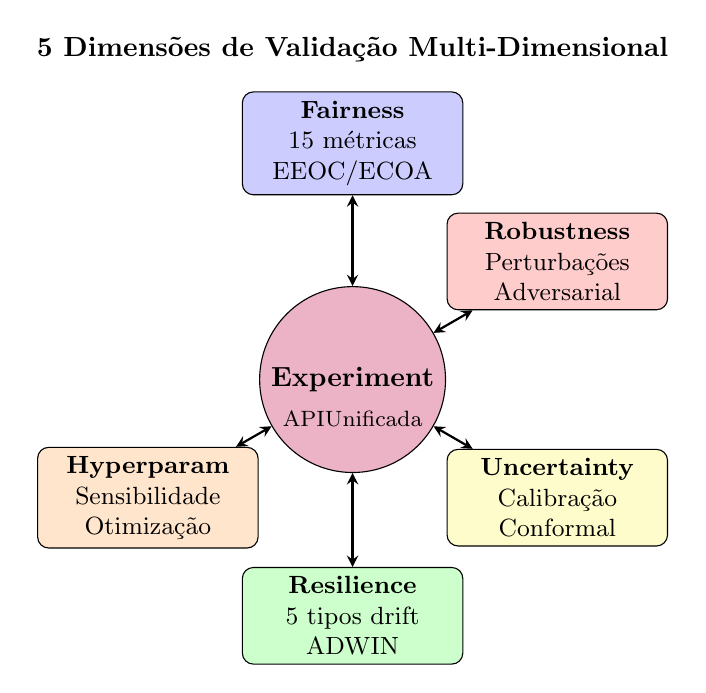
\begin{tikzpicture}[
    dimension/.style={rectangle, draw, rounded corners, minimum width=2.8cm, minimum height=1.2cm, align=center, font=\small, fill=#1},
    arrow/.style={->, >=stealth, thick}
]

% Central component
\node[circle, draw, fill=purple!30, minimum size=2cm, font=\bfseries] (exp) at (0,0) {Experiment};

% 5 dimensions around
\node[dimension=blue!20] (fairness) at (0,3) {\textbf{Fairness}\\15 métricas\\EEOC/ECOA};
\node[dimension=red!20] (robust) at (2.6,1.5) {\textbf{Robustness}\\Perturbações\\Adversarial};
\node[dimension=yellow!20] (uncertain) at (2.6,-1.5) {\textbf{Uncertainty}\\Calibração\\Conformal};
\node[dimension=green!20] (resilience) at (0,-3) {\textbf{Resilience}\\5 tipos drift\\ADWIN};
\node[dimension=orange!20] (hyperparam) at (-2.6,-1.5) {\textbf{Hyperparam}\\Sensibilidade\\Otimização};

% Arrows
\draw[arrow, <->] (exp) -- (fairness);
\draw[arrow, <->] (exp) -- (robust);
\draw[arrow, <->] (exp) -- (uncertain);
\draw[arrow, <->] (exp) -- (resilience);
\draw[arrow, <->] (exp) -- (hyperparam);

% Central label
\node[font=\footnotesize] at (0,-0.5) {API\\Unificada};

% Title
\node[font=\bfseries] at (0,4.2) {5 Dimensões de Validação Multi-Dimensional};

\end{tikzpicture}
\caption{As cinco dimensões de validação integradas no DeepBridge através de uma API unificada. Cada dimensão é gerenciada por um Test Manager especializado, coordenado pelo Experiment orchestrator.}
\label{fig:validation_dimensions}
\end{figure}
